% Options for packages loaded elsewhere
\PassOptionsToPackage{unicode}{hyperref}
\PassOptionsToPackage{hyphens}{url}
%
\documentclass[
]{article}
\usepackage{amsmath,amssymb}
\usepackage{iftex}
\ifPDFTeX
  \usepackage[T1]{fontenc}
  \usepackage[utf8]{inputenc}
  \usepackage{textcomp} % provide euro and other symbols
\else % if luatex or xetex
  \usepackage{unicode-math} % this also loads fontspec
  \defaultfontfeatures{Scale=MatchLowercase}
  \defaultfontfeatures[\rmfamily]{Ligatures=TeX,Scale=1}
\fi
\usepackage{lmodern}
\ifPDFTeX\else
  % xetex/luatex font selection
\fi
% Use upquote if available, for straight quotes in verbatim environments
\IfFileExists{upquote.sty}{\usepackage{upquote}}{}
\IfFileExists{microtype.sty}{% use microtype if available
  \usepackage[]{microtype}
  \UseMicrotypeSet[protrusion]{basicmath} % disable protrusion for tt fonts
}{}
\makeatletter
\@ifundefined{KOMAClassName}{% if non-KOMA class
  \IfFileExists{parskip.sty}{%
    \usepackage{parskip}
  }{% else
    \setlength{\parindent}{0pt}
    \setlength{\parskip}{6pt plus 2pt minus 1pt}}
}{% if KOMA class
  \KOMAoptions{parskip=half}}
\makeatother
\usepackage{xcolor}
\usepackage[margin=1in]{geometry}
\usepackage{graphicx}
\makeatletter
\def\maxwidth{\ifdim\Gin@nat@width>\linewidth\linewidth\else\Gin@nat@width\fi}
\def\maxheight{\ifdim\Gin@nat@height>\textheight\textheight\else\Gin@nat@height\fi}
\makeatother
% Scale images if necessary, so that they will not overflow the page
% margins by default, and it is still possible to overwrite the defaults
% using explicit options in \includegraphics[width, height, ...]{}
\setkeys{Gin}{width=\maxwidth,height=\maxheight,keepaspectratio}
% Set default figure placement to htbp
\makeatletter
\def\fps@figure{htbp}
\makeatother
\setlength{\emergencystretch}{3em} % prevent overfull lines
\providecommand{\tightlist}{%
  \setlength{\itemsep}{0pt}\setlength{\parskip}{0pt}}
\setcounter{secnumdepth}{-\maxdimen} % remove section numbering
\usepackage{booktabs}
\usepackage{longtable}
\usepackage{array}
\usepackage{multirow}
\usepackage{wrapfig}
\usepackage{float}
\usepackage{colortbl}
\usepackage{pdflscape}
\usepackage{tabu}
\usepackage{threeparttable}
\usepackage{threeparttablex}
\usepackage[normalem]{ulem}
\usepackage{makecell}
\usepackage{xcolor}
\ifLuaTeX
  \usepackage{selnolig}  % disable illegal ligatures
\fi
\usepackage{bookmark}
\IfFileExists{xurl.sty}{\usepackage{xurl}}{} % add URL line breaks if available
\urlstyle{same}
\hypersetup{
  pdftitle={Coding Assumptions},
  hidelinks,
  pdfcreator={LaTeX via pandoc}}

\title{Coding Assumptions}
\author{}
\date{\vspace{-2.5em}}

\begin{document}
\maketitle

The analysis of Project XX-XX required developing General Transit Feed
Specification (GTFS) files to model the proposed fixed route bus
service.

The following sections of this report describe service characteristics
encoded into the GTFS files.

\subsection{Alignment and Service
Characteristic}\label{alignment-and-service-characteristic}

The project provides new service along two alignments between Shady
Grove Metro East and Traville Transit Center.

\begin{itemize}
\item
  \textbf{Pink Line:} Establishes a connection from the bustling Shady
  Grove corridor to the Life Sciences Center via Medical Center Drive,
  with a round-trip travel time estimate is 66:30.
\item
  \textbf{Lime Line:} Provides an express service along I-370 to RIO,
  Crown Farm, and central locations within the Life Science Center, with
  a round-trip travel time estimate of 51:43.
\end{itemize}

Dedicated bus lanes will be constructed along existing curbside lanes to
enhance travel times and improve reliability. Right-turning vehicles
will be permitted to use these lanes at designated intersections.
Transit Signal Priority (TSP) will be implemented at key intersections
along the Pink Line.

The following maps depicts station locations and route alignment
developed to calculate travel distances and travel times for coding the
proposed service into a GTFS feed.

\begin{verbatim}
## Loading basemap 'light_only_labels' from map service 'carto'...
\end{verbatim}

\begin{verbatim}
## Loading basemap 'light_no_labels' from map service 'carto'...
\end{verbatim}

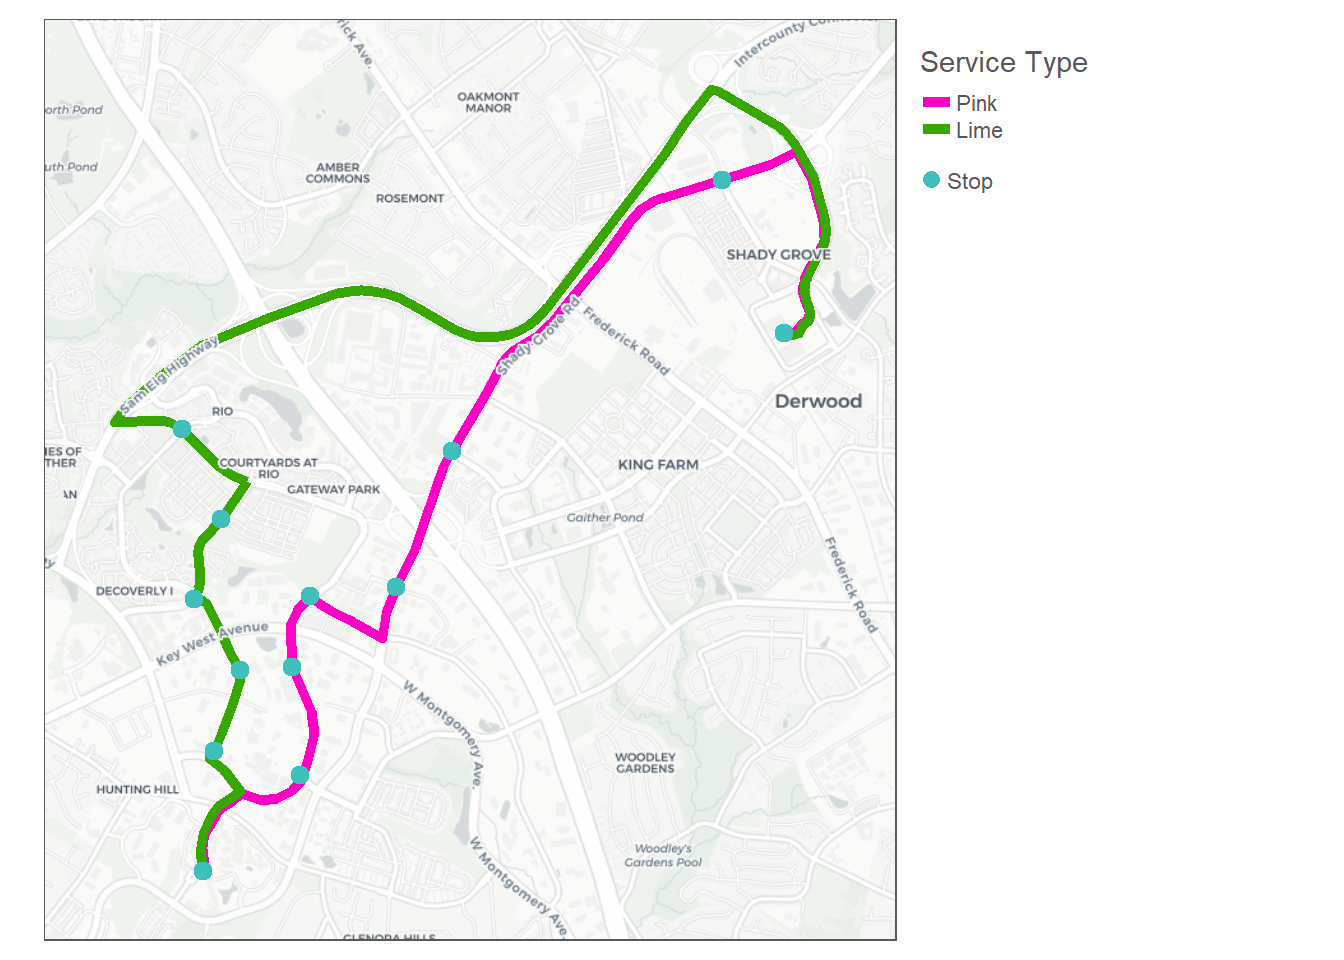
\includegraphics{coding-assumptions_files/figure-latex/unnamed-chunk-2-1.pdf}

Details of how the proposed service is represented in GTFS are provided
below by describing four key tables in the feed: Stops.txt, Trips.txt,
Stop\_times.txt, and Frequencies.txt. Other tables in the new XX-XX feed
are based on standard tables defined in the Chapter 30 Transit
Accessibility Scoring Guide
(``\href{https://accessdocs.readthedocs.io/en/latest/quality-assurance.html\#gtfs-feed-validation}{GTFS
feed validation}'' section) and are not described here.

\subsection{Attributes}\label{attributes}

The attributes of the base multimodal network were modified through the
addition of the newly developed GTFS feed modeling Project XX-XX. The
details of how Project XX-XX was represented in GTFS are provided below
by describing four key tables of the feeds: Stops.txt, Trips.txt,
Stop\_times.txt, and Frequencies.txt.

Other tables in the new project feed are based on standard tables
defined in the Chapter 30 Transit Accessibility Scoring Guide
(``Standard GTFS Tables'' section) and are not described here.

\subsubsection{Stops.txt}\label{stops.txt}

\textbf{Table 1. Stops Table}

\begin{table}
\centering
\begin{tabular}[t]{l|l|l|l|r|r}
\hline
stop\_id & stop\_code & stop\_name & stop\_desc & stop\_lat & stop\_lon\\
\hline
pink1 & pink1 & SHADY GROVE METRO STATION - EAST (Bay F) & Shady Grove Metro Station - East & 39.12078 & -77.16335\\
\hline
pink2 & pink2 & SHADY GROVE RD AT CRABBS BRANCH WAY & Westside at Shady Grove & 39.12878 & -77.16753\\
\hline
pink3 & pink3 & SHADY GROVE RD AT CHOKE CHERRY RD & Rockville - Choke Cherry Crossing & 39.11463 & -77.18572\\
\hline
pink4 & pink4 & SHADY GROVE RD AT CORPORATE BLVD & Shady Grove Corporate Center & 39.10752 & -77.18947\\
\hline
pink5 & pink5 & OMEGA DR AT RESEARCH BLVD & Crown - East & 39.10706 & -77.19523\\
\hline
pink6 & pink6 & MEDICAL CENTER DR AT JHU & Life Sci - East & 39.10337 & -77.19646\\
\hline
pink7 & pink7 & MEDICAL CENTER DR AT MEDICAL CENTER WAY & Shady Grove Medical Center- South & 39.09771 & -77.19590\\
\hline
pink8 & pink8 & TRAVILLE TRANSIT CENTER UNIVERSITY OF SHADY GROVE & Traville Transit Center & 39.09273 & -77.20242\\
\hline
lime1 & lime1 & SHADY GROVE METRO STATION - EAST (Bay E) & Shady Grove Metro Station - East & 39.12078 & -77.16335\\
\hline
lime2 & lime2 & FIELDS RD AT RIO BLVD & Downtown Crown/Rio Washingtonian Center & 39.11578 & -77.20383\\
\hline
lime3 & lime3 & DECOVERLY DR AT CROWN PARK AVE & Crown - Central & 39.11111 & -77.20120\\
\hline
lime4 & lime4 & DIAMOND DR AT DECOVERLY DR & Decoverly & 39.10693 & -77.20302\\
\hline
lime5 & lime5 & BROSCHART RD AT JHU & Life Sci - West & 39.10320 & -77.19993\\
\hline
lime6 & lime6 & BROSCHART RD AT MEDICAL CENTER WAY & Shady Grove Medical Center - West & 39.09899 & -77.20167\\
\hline
lime7 & lime7 & TRAVILLE TRANSIT CENTER UNIVERSITY OF SHADY GROVE & Traville Transit Center & 39.09273 & -77.20242\\
\hline
\end{tabular}
\end{table}

\subsubsection{Trips.txt (vehicle-trip
enumeration)}\label{trips.txt-vehicle-trip-enumeration}

The trips file represents a single route with a seven-day travel
profile. The scoring methodology is based around peak AM travel times.
The feed was only developed to represent this time period and the
associated frequencies and characteristics.

\textbf{Table 2. Trips Table}

\begin{table}
\centering
\begin{tabular}[t]{l|l|l|l|l|l|l|l|l|l}
\hline
route\_id & service\_id & trip\_id & trip\_headsign & trip\_short\_name & direction\_id & block\_id & shape\_id & wheelchair\_accessible & bikes\_allowed\\
\hline
gstn\_express & MTWTF & pink\_sb & NA & NA & NA & NA & NA & NA & NA\\
\hline
gstn\_express & MTWTF & pink\_nb & NA & NA & NA & NA & NA & NA & NA\\
\hline
gstn\_express & MTWTF & lime\_sb & NA & NA & NA & NA & NA & NA & NA\\
\hline
gstn\_express & MTWTF & lime\_nb & NA & NA & NA & NA & NA & NA & NA\\
\hline
\end{tabular}
\end{table}

\subsubsection{Stop\_times.txt (transit
schedule)}\label{stop_times.txt-transit-schedule}

The stop times table was developed by determining an average travel
speed based on the travel time and approximate length of the line.

\textbf{Table 3. Stops Times Table}

\begin{table}
\centering
\begin{tabular}[t]{l|l|l|l|r}
\hline
trip\_id & arrival\_time & departure\_time & stop\_id & stop\_sequence\\
\hline
pink\_sb & 06:01:00 & 06:01:00 & pink1 & 1\\
\hline
pink\_sb & 06:09:50 & 06:09:50 & pink2 & 2\\
\hline
pink\_sb & 06:17:37 & 06:17:37 & pink3 & 3\\
\hline
pink\_sb & 06:20:13 & 06:20:13 & pink4 & 4\\
\hline
pink\_sb & 06:22:49 & 06:22:49 & pink5 & 5\\
\hline
pink\_sb & 06:24:54 & 06:24:54 & pink6 & 6\\
\hline
pink\_sb & 06:26:27 & 06:26:27 & pink7 & 7\\
\hline
pink\_sb & 06:34:15 & 06:34:15 & pink8 & 8\\
\hline
pink\_nb & 06:01:00 & 06:01:00 & pink8 & 1\\
\hline
pink\_nb & 06:08:48 & 06:08:48 & pink7 & 2\\
\hline
pink\_nb & 06:10:21 & 06:10:21 & pink6 & 3\\
\hline
pink\_nb & 06:12:26 & 06:12:26 & pink5 & 4\\
\hline
pink\_nb & 06:15:02 & 06:15:02 & pink4 & 5\\
\hline
pink\_nb & 06:17:37 & 06:17:37 & pink3 & 6\\
\hline
pink\_nb & 06:25:25 & 06:25:25 & pink2 & 7\\
\hline
pink\_nb & 06:34:15 & 06:34:15 & pink1 & 8\\
\hline
lime\_sb & 06:01:00 & 06:01:00 & lime1 & 1\\
\hline
lime\_sb & 06:09:58 & 06:09:58 & lime2 & 2\\
\hline
lime\_sb & 06:17:53 & 06:17:53 & lime3 & 3\\
\hline
lime\_sb & 06:20:31 & 06:20:31 & lime4 & 4\\
\hline
lime\_sb & 06:23:09 & 06:23:09 & lime5 & 5\\
\hline
lime\_sb & 06:25:16 & 06:25:16 & lime6 & 6\\
\hline
lime\_sb & 06:26:51 & 06:26:51 & lime7 & 7\\
\hline
lime\_nb & 06:01:00 & 06:01:00 & lime7 & 1\\
\hline
lime\_nb & 06:02:35 & 06:02:35 & lime6 & 2\\
\hline
lime\_nb & 06:04:42 & 06:04:42 & lime5 & 3\\
\hline
lime\_nb & 06:07:20 & 06:07:20 & lime4 & 4\\
\hline
lime\_nb & 06:09:58 & 06:09:58 & lime3 & 5\\
\hline
lime\_nb & 06:17:53 & 06:17:53 & lime2 & 6\\
\hline
lime\_nb & 06:26:51 & 06:26:51 & lime1 & 7\\
\hline
\end{tabular}
\end{table}

\subsubsection{Frequencies.txt (frequency of recurring
trips)}\label{frequencies.txt-frequency-of-recurring-trips}

A frequencies table was developed to model the headways of the line
during weekday AM peak travel times. The table defines a start and end
time for a headway, with each headway associated with a trip ID. The
headways are provided in seconds. The trip IDs link the headway times to
the individual trips that comprise the route described in the trips.txt
file. When frequencies table is used, the stop times file defines a
template of stop sequences and travel times between stops, and the
frequencies table defines the interval of recurrence for each trip
following the stop times template.

\textbf{Table 4. Frequencies Table}

\begin{table}
\centering
\begin{tabular}[t]{l|l|l|r|l}
\hline
trip\_id & start\_time & end\_time & headway\_secs & exact\_times\\
\hline
pink\_sb & 06:00:00 & 10:00:00 & 600 & NA\\
\hline
pink\_nb & 06:00:00 & 10:00:00 & 600 & NA\\
\hline
lime\_sb & 06:00:00 & 10:00:00 & 900 & NA\\
\hline
lime\_nb & 06:00:00 & 10:00:00 & 900 & NA\\
\hline
\end{tabular}
\end{table}

\subsubsection{Network}\label{network}

The following maps depict the GTFS feed for both base service as well as
proposed service represented as a routable network. While the alignment
was used to develop route distances and speeds, the resulting
GTFS-derived network represents transit service as straight lines
between stops, with the associated scheduling information that was built
around the specific alignments associated with each segment.

\textbf{Figure 2. Base Network}

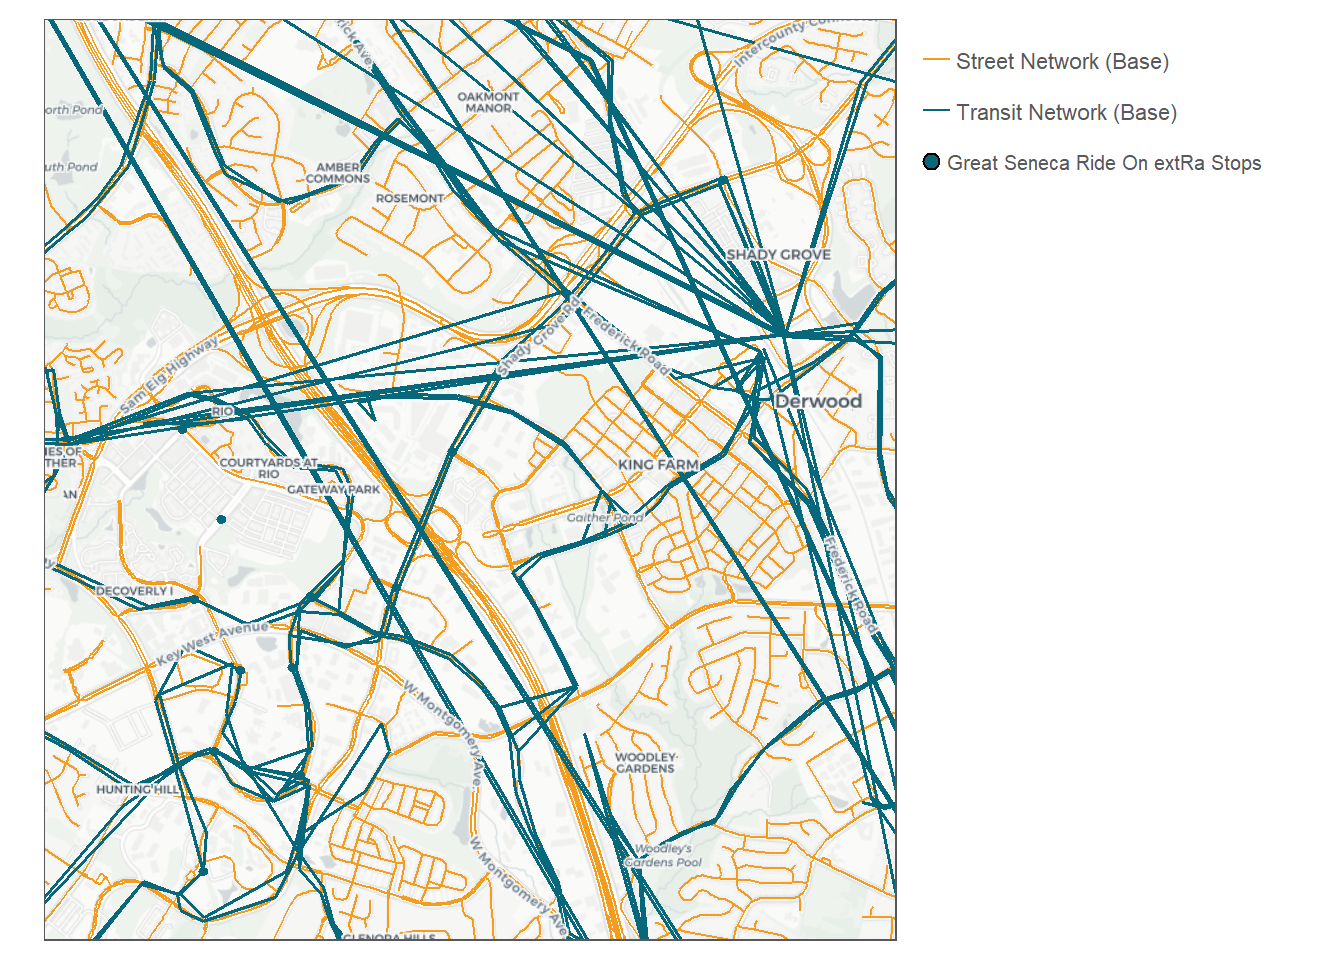
\includegraphics{coding-assumptions_files/figure-latex/base network-1.pdf}

\textbf{Figure 3. Build Network}

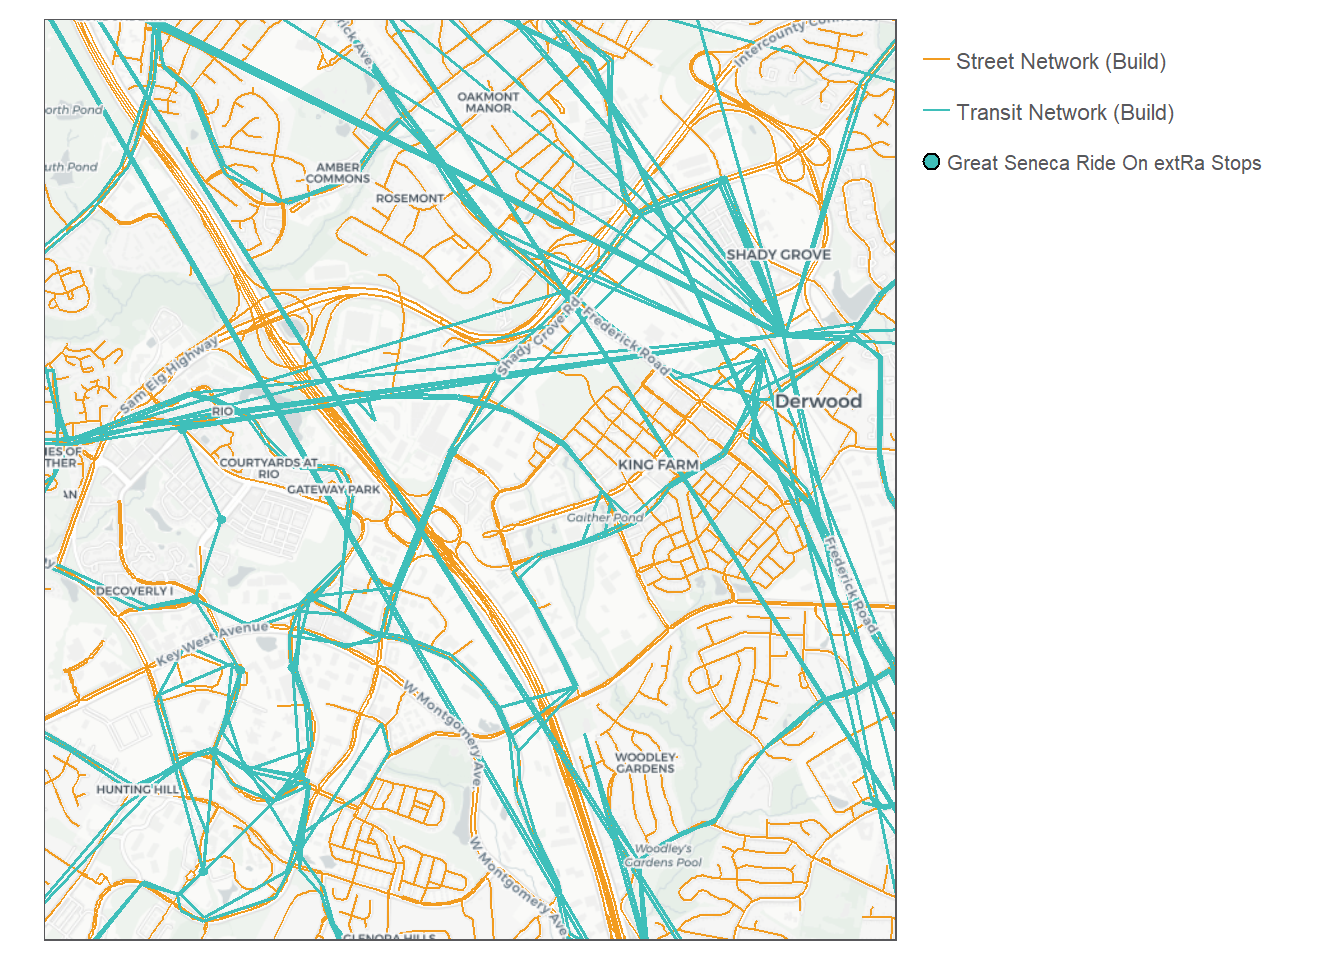
\includegraphics{coding-assumptions_files/figure-latex/build network-1.pdf}

\end{document}
